\section{Results}\label{Sec:Results}

\begin{itemize}

\item Organize material and present results.

\item Use tables, figures (but prefer visual presentation):
\begin{itemize}
\item Tables and figures should supplement (and not duplicate) the
text.

\item Tables and figures should be provided with
legends.\\
{\it Figure \ref{Fig:Resids} shows how to include and reference
graphics. The graphic must be labelled before. Files must be in
\texttt{.eps} format.}

\begin{figure}[ht]
\begin{center}
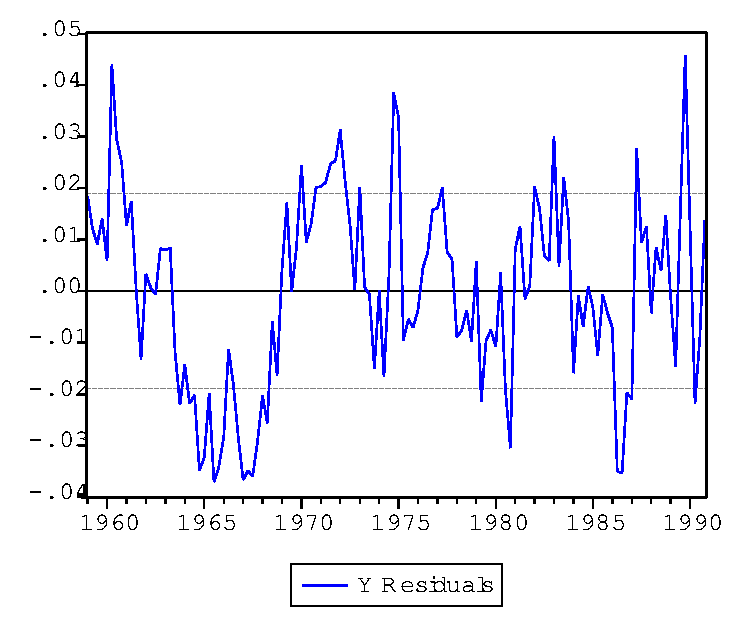
\includegraphics[scale=0.5,angle=0]{graph}
\caption{Estimated residuals from model XXX. ...}
\label{Fig:Resids}
\end{center}
\end{figure}

\item Tables and graphics may appear in the text or in
the appendix, especially if there are many simulation results
tabulated, but is also depends on the study and number of tables resp.
figures. The key graphs and tables must appear in
the text!
\end{itemize}

\item Latex is really good at rendering formulas:\\
{\it Equation (\ref{Eq:SpecDens}) represents the ACs of a stationary
stochastic process:
\begin{equation}
f_y(\lambda) = (2\pi)^{-1} \sum_{j=-\infty}^{\infty}
\gamma_j e^{-i\lambda j}
=(2\pi)^{-1}\left(\gamma_0 + 2 \sum_{j=1}^{\infty}
\gamma_j \cos(\lambda j)\right)
            \label{Eq:SpecDens}
\end{equation}
where $i=\sqrt{-1}$ is the imaginary unit, $\lambda \in [-\pi,
\pi]$ is the frequency and the $\gamma_j$ are the autocovariances
of $y_t$.}

\newpage

\item Discuss results:
\begin{itemize}
\item Do the results support or do they contradict economic theory ?
\item What does the reader learn from the results?
\item Try to give an intuition for your results.
\item Provide robustness checks.
\item Compare to previous research.
\end{itemize}
\end{itemize}

\subsection{Sample Preparation}
FFPE <-> library concentration

Pictures of Bioanalyzer

\begin{figure}[!tbp]
  \centering
  \subfloat[Overlayed Electropherograms of Four Representative Libraries Prepared with Agilent Haloplex CSC]{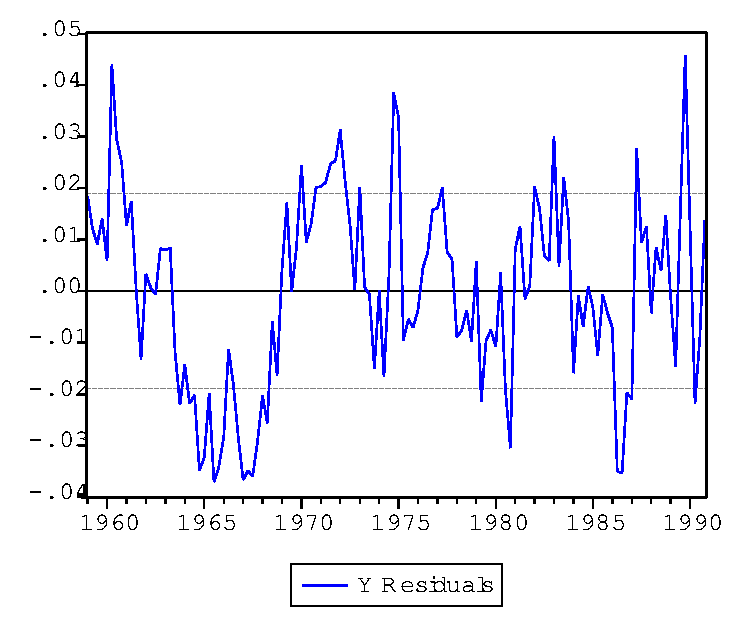
\includegraphics[width=0.45\textwidth]{graph.pdf}\label{fig:f1}}
  \hfill
  \subfloat[Overlayed Electropherograms of Four Representative Libraries Prepared with Illumina TST15 (MixA \& MixB)]{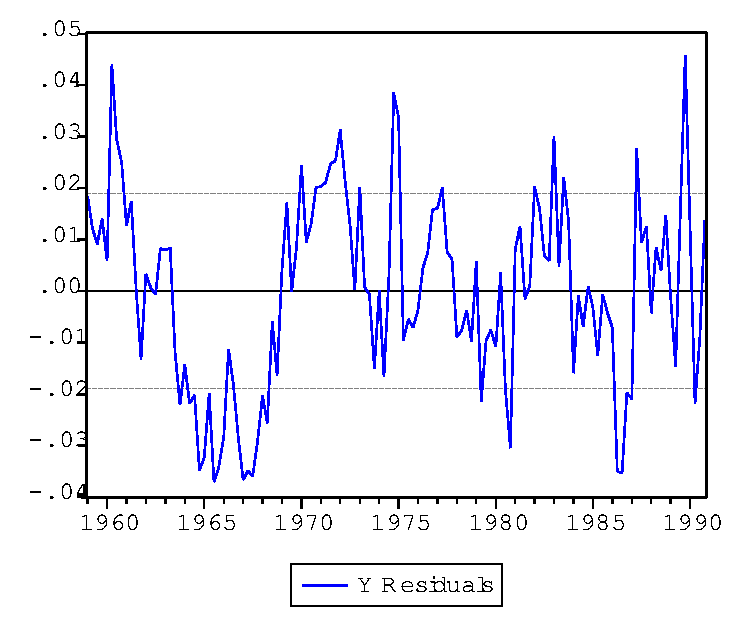
\includegraphics[width=0.45\textwidth]{graph.pdf}\label{fig:f2}}
  \caption{Comparison of Agilent Bioanalyzer Electropherograms}
\end{figure}

\subsection{NGS Data Quality}

Illumina Sequencing Viewer

\begin{table}[!htbp]
    \caption[ISV]{Comparison of Run Parameters (Averaged) of Sequencing Runs with Haloplex CSC \& TST15 Sample Preparation}
    \centering
    \begin{tabular}{ |p{4cm}||p{4cm}||p{4cm}|}
    \hline
    Parameter & Haloplex CSC & TST15 \\ \hline \hline
    Yield total (Gb) & 3.7 & 7.37 \\ \hline
    \% \textgreater Q30 & 93.8 & 82.355 \\ \hline
    Cluster Density PF (k/mm2) & 1084 & 1180  \\ \hline
    Cluster Density PF (%) & 85.95 & 79.95  \\ \hline
  \end{tabular}
\end{table}

FASTQC


\begin{minipage}{0.5\textwidth}
The Samtools Flagstat command was used to determine some basic BAM statistics of BAM
files of samples prepared with the respective library preparations and processed with
the mentioned bioinformatic pipelines. \ref{table:samtools_flagstat} shows the
averaged result of these statistics. Considering the recommended pipelines, Haloplex
CSC data, analyzed with Agilent's SureCall software, has a higher percentage (91\%) of mapped
reads when compared to Illumina's BaseSpace TruSight Tumor 15 App (62.9\%). Data analysis
with the recommended SureCall design includes a steps where mates are fixed, but they
are not stitched together. Therefore no reads are considered as being paired. The TST15 app
in contrast includes a read stitching step and 58\% are considered as properly paired.
This means that of the 62.6\% of mapped reads, 4.2\% are not properly paired. 3.8\%
of reads processed with the TST15 online App are considered to be singletons, whereas
only 1.8\% of reads processed with the SureCall software are considered as singletons.
\end{minipage}
\hfill
\begin{minipage}{0.5\textwidth}
\captionof{table}{Your caption here}
\begin{tabular}{p{3cm} p{1.5cm} p{1.5cm}}\\
\hline
Parameter & Haloplex CSC & TST15 \\
\hline
\% mapped & 91 & 62.6 \\
\% paired & 0 & 58.7 \\
\% singletons & 1.8 & 3.8 \\
\label{samtools_flagstat}
\end{tabular}
\end{minipage}

\subsection{Coverage Analysis}

Coverage Distribution TST15 vs Haloplex

Coverage Distribution per Patient (check if correlation IQR with dCt)

Coverage Distribution per Amplicon (check if some have always lower coverage, check if some failed)
\begin{figure}[!tbp]
  \centering
  \subfloat[Agilent Haloplex ClearSeq Cancer]{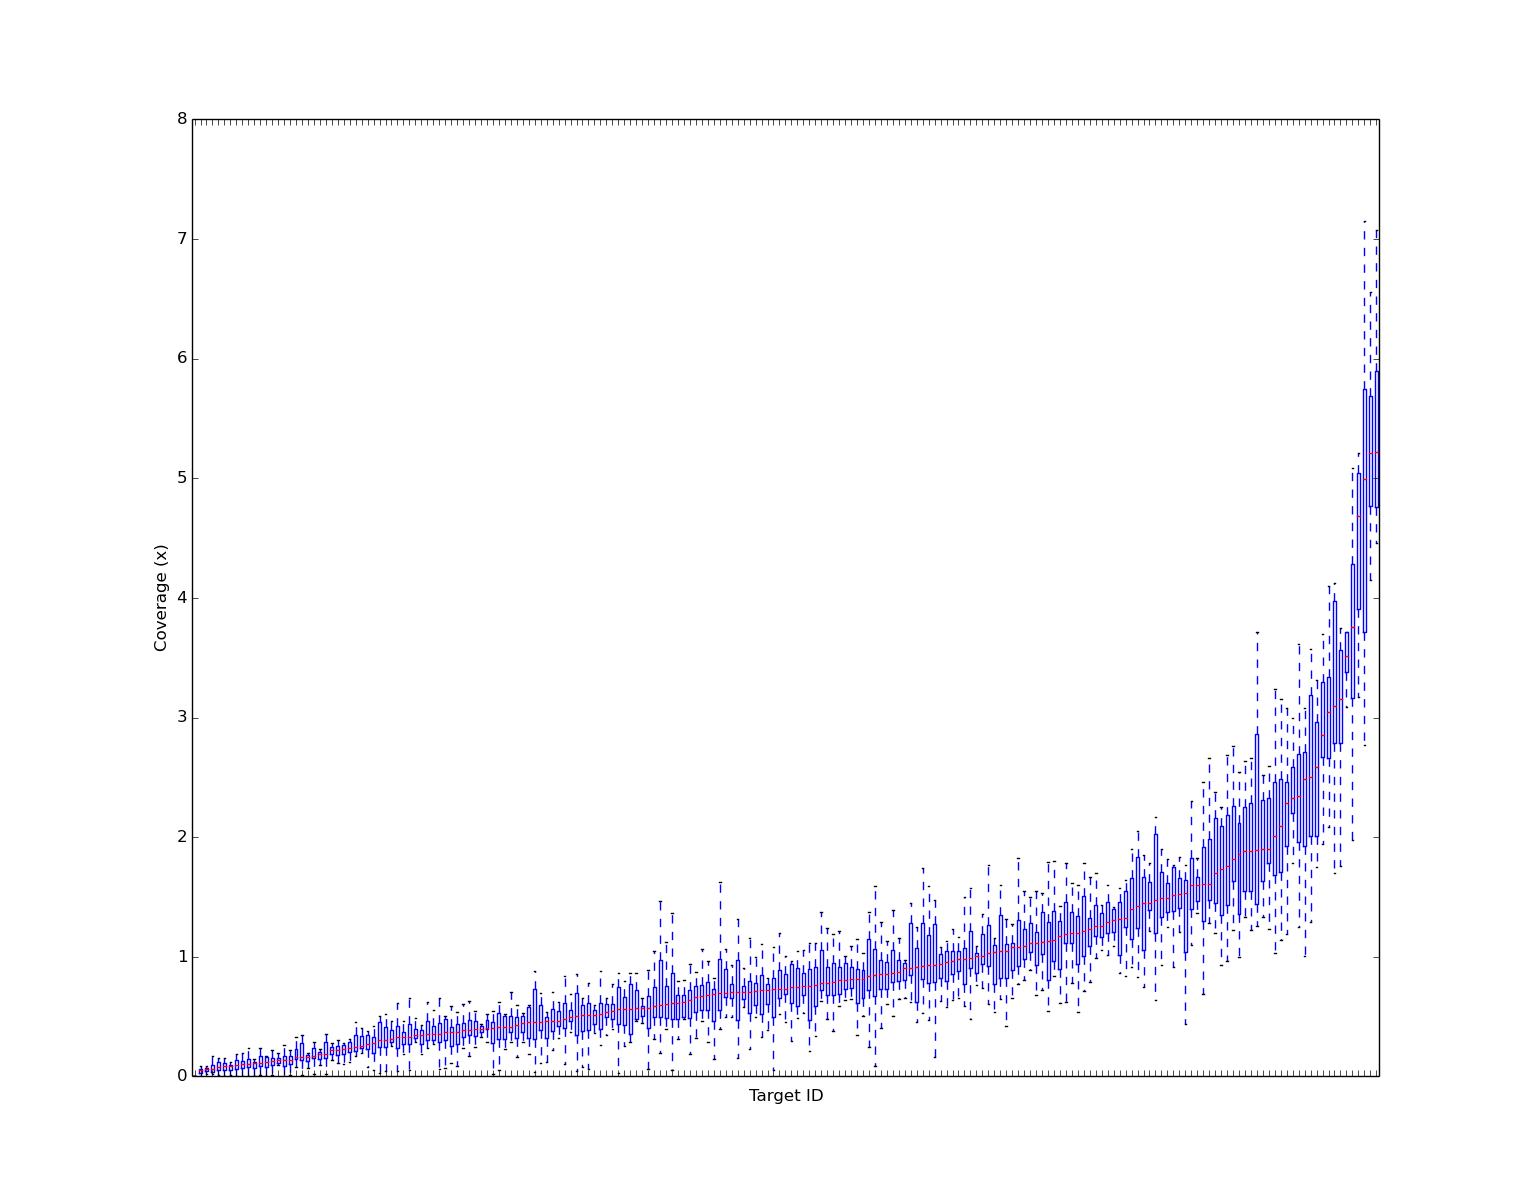
\includegraphics[width=0.45\textwidth]{distribution_amplicons_hap_csc.png}\label{fig:amp_dist_hpx}}
  \hfill
  \subfloat[Illumina TruSight Tumor 15]{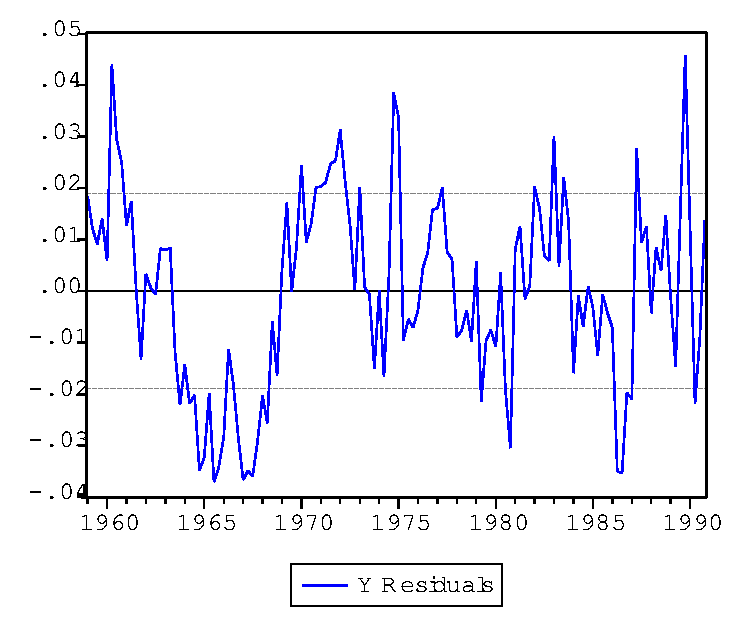
\includegraphics[width=0.45\textwidth]{graph.pdf}\label{fig:amp_dist_tst}}
  \caption{Comparison of Coverage Distributions per Amplicon}
\end{figure}

% Merge TST15 MixA & MixB together in one figure.
% Try to extract median values out of boxplots; new figure with these points
% -> some kind of trend line. The sooner it gets to a normalized coverage value of 1,
% the better.

% Looks like TST15 are better than Haloplex. But problem in TST: some EGFR & KRAS
% have low distributions.

%Doo the same for EGFR; KRAS; NRAS; BRAF

Failed Amplicon Counter

\begin{minipage}{0.5\textwidth}
\captionof{table}{Failed Amplicons in Agilent Haloplex ClearSeq Cancer}
\begin{tabular}{p{1.5cm} p{1.5cm} p{1.5cm}}\\
\hline
Amplicon & Coverage Failed & No of Samples \\
\hline
ATM_14 & 1 & all \\
Bla & 200 & 9 \\
Blabla & 500 & 5 \\
\label{failed_hpx}
\end{tabular}
\end{minipage}
\hfill
\begin{minipage}{0.5\textwidth}
\captionof{table}{Your caption here}
\begin{tabular}{p{3cm} p{1.5cm} p{1.5cm}}\\
\hline
Amplicon & Coverage Failed & No of Samples \\
\hline
ATM_14 & 1 & all \\
Bla & 200 & 9 \\
Blabla & 500 & 5 \\
\label{failed_tst}
\end{tabular}
\end{minipage}

Fragmentation <-> Coverage?
% Scatter plot: dCt vs normalized coverage (median / IQR ???)

(GATK CallableLoci)
(GATK CountLoci???)
(GATK FindCoveredIntervals)

On-off target; Enrichment Efficiency TST15 vs Haloplex

Coverage across genome, check where there is coverage

Strandedness?

GATK DepthOfCoverage???

\subsection{Variant Calling Algorithm Comparison}
Detection of Known Single Nucleotide Variants and Deletions

Which should be found?

Which have not been found? Why?

\begin{table}[!htbp]
  \caption[known_variants]{Known Variant Detection}
  \centering
    \begin{tabular}{ |p{4cm}||p{4cm}||p{4cm}|}
    \hline
    Gene & Chr & Pos & Ref & Alt & Haloplex & TST15 \\ \hline \hline
    Yield total (Gb) & 3.7 & 7.37 \\ \hline
    \% \textgreater Q30 & 93.8 & 82.355 \\ \hline
    Cluster Density PF (k/mm2) & 1084 & 1180  \\ \hline
    Cluster Density PF (%) & 85.95 & 79.95  \\ \hline
  \end{tabular}
\end{table}

MuTect

VarScan

GATK HaplotypeCaller

SomVarIUS????????
Freebayes????????
Vardict???????

SureCall & TST15

GATK SelectVariants
GATK VariantFiltration
GATK VariantEval
GATK ValidateVariants

More C>T ?
